\section{Sở GD Bắc Ninh -- Liên trường NH: 2025--2026}

\noindent\textbf{PHẦN I. Câu trắc nghiệm nhiều phương án lựa chọn.} Thí sinh trả lời từ câu $1$ đến câu $12$. Mỗi câu thí sinh chỉ chọn một phương án.
\setcounter{ex}{0}
\begin{ex} %[2D1H3-1] %Câu 1
	Giá trị nhỏ nhất của hàm số $y=(x-3)^2 \mathrm{e}^x$ trên đoạn $[0;2]$ bằng
	\choice
	{$9$}
	{$\mathrm{e}^2$}
	{$0$}
	{\True $4\mathrm{e}$}
	\loigiai{
		Hàm số $y=(x-3)^2 \mathrm{e}^x$ liên tục trên đoạn $[0;2]$.\\
		Ta có $y'=2(x-3)\mathrm{e}^x+(x-3)^2 \mathrm{e}^x = \mathrm{e}^x(x-3)(x-1)$.\\
		Khi đó $y'=0 \Leftrightarrow \mathrm{e}^x(x-3)(x-1)=0 \Leftrightarrow \hoac{&x=3 \\ &x=1 \in [0;2]}$.\\
		Do đó $y(0)=9$; $y(1)=4\mathrm{e}$; $y(2)=\mathrm{e}^2$.\\
		Vậy giá trị nhỏ nhất của hàm số $y=(x-3)^2 \mathrm{e}^x$ trên đoạn $[0;2]$ bằng $y(1)=4\mathrm{e}$.
	}
\end{ex}

\begin{ex} %[1D6H4-5] %Câu 2
	Bất phương trình $1+\log_2(x-2) > \log_2(x^2-3x+2)$ có tập nghiệm là
	\choice
	{\True $S=(2;3)$}
	{$S=(3;+\infty)$}
	{$S=(2;+\infty)$}
	{$S=(1;3)$}
	\loigiai{
		Điều kiện $\heva{& x-2>0 \\ & x^2-3x+2>0} \Leftrightarrow \heva{& x>2 \\ & \hoac{&x<1 \\ &x>2}} \Leftrightarrow x>2$.\\
		Bất phương trình $1+\log_2(x-2) > \log_2(x^2-3x+2)$
		\begin{align*}
			&\Leftrightarrow \log_2 2 + \log_2(x-2) > \log_2(x^2-3x+2) \\
			&\Leftrightarrow \log_2 2(x-2) > \log_2(x^2-3x+2) \\
			&\Rightarrow 2(x-2) > x^2-3x+2 \\
			&\Leftrightarrow x^2-5x+6 < 0 \\
			&\Leftrightarrow 2 < x < 3
		\end{align*}
		Kết hợp điều kiện ta được $2 < x < 3$. Vậy tập nghiệm là $S=(2;3)$.
	}
\end{ex}

\begin{ex} %[2D1H1-2] %Câu 3
	Cho hàm số $y=f(x)$ xác định, có đạo hàm trên $\mathbb{R}$ và $f'(x)$ có đồ thị như hình vẽ.
	\begin{center}
		\begin{tikzpicture}[scale=1, font=\footnotesize, line join=round, line cap=round, >=stealth]
			\draw[->] (-3.5,0)--(1,0) node[below]{$x$};
			\draw[->] (0,-2.5)--(0,2) node[right]{$y$};
			\draw[fill=blue] (0,0) coordinate(O) circle (1pt) node[above left]{$O$};
			\clip (-3.5,-2.5) rectangle (2,2);
			\draw[domain=-3.5:1, samples=200] plot (\x,{-(\x+3)*(\x+2)*(\x)^2})node[above]{$f'(x)$};
			\foreach \x/\y in {-3/-150, -2/-145}{\fill[blue] (\x,0) circle (1pt); \node[shift={(\y:3.5mm)}] at (\x,0) {$\x$};}
		\end{tikzpicture}
	\end{center}
	Mệnh đề nào sau đây đúng?
	\choice
	{Hàm số $y=f(x)$ nghịch biến trên khoảng $(-2;+\infty)$}
	{Hàm số $y=f(x)$ đồng biến trên khoảng $\left(-\dfrac{1}{2};0\right)$}
	{Hàm số $y=f(x)$ nghịch biến trên khoảng $\left(-\dfrac{5}{2};-2\right)$}
	{\True Hàm số $y=f(x)$ nghịch biến trên khoảng $(-\infty;-3)$}
	\loigiai{
		Dựa vào đồ thị, $f'(x)$ cắt trục hoành tại $x=-3; x=-2; x=0$ (nghiệm kép).
		Nên ta có bảng xét dấu như sau:
		\begin{center}
			
\begin{tikzpicture}
				\tkzTabInit[lgt=1.2, espcl=2.5, deltacl=0.5]
				{$x$ / 0.7, $f'(x)$ / 0.7}
				{$-\infty$, $-3$, $-2$, $0$, $+\infty$}
				\tkzTabLine{ , -, 0, +, 0, -, 0, -, }
			\end{tikzpicture}
		\end{center}
		Dựa vào bảng xét dấu, hàm số $y=f(x)$ nghịch biến trên khoảng $(-\infty;-3)$.
	}
\end{ex}

\begin{ex} %[2D1N2-2] %Câu 4
	Cho hàm số $y=f(x)$ có bảng biến thiên sau:
	\begin{center}
		
\begin{tikzpicture}
			\tkzTabInit[lgt=1.2, espcl=2.5, deltacl=0.5]
			{$x$ / 0.7, $y'$ / 0.7, $y$ / 2}
			{$-\infty$, $-3$, $-2$, $1$, $+\infty$}
			\tkzTabLine{ , -, 0, +, d, +, 0, -, }
			\tkzTabVar{+ / $+\infty$, - / $5$, +D- / $+\infty$ / $-\infty$, + / $0$, - / $-\infty$}
		\end{tikzpicture}
	\end{center}
	Giá trị cực đại của hàm số $y=f(x)$ là
	\choice
	{$1$}
	{$-3$}
	{$5$}
	{\True $0$}
	\loigiai{
		Dựa vào bảng biến thiên, giá trị cực đại của hàm số $y=f(x)$ là $0$.
	}
\end{ex}

\begin{ex} %[2D1H5-1] %Câu 5
	Đường cong trong hình bên là đồ thị của hàm số nào dưới đây?
	\begin{center}
		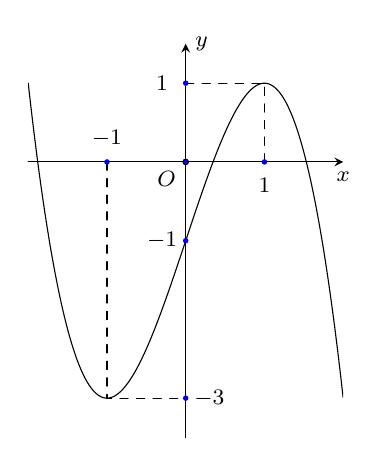
\begin{tikzpicture}[scale=1, font=\footnotesize, line join=round, line cap=round, >=stealth]
			\draw[->] (-2,0)--(2,0) node[below]{$x$};
			\draw[->] (0,-3.5)--(0,1.5) node[right]{$y$};
			\draw[fill=blue] (0,0) coordinate(O) circle (1pt) node[below left]{$O$};
			\clip (-2,-3.5) rectangle (2,1.5);
			\draw[domain=-2:2, samples=200] plot (\x,{-(\x)^3+3*(\x)-1});
			\foreach \x/\y in {-1/-3, 1/1}{\draw[dashed] (\x,0)--(\x,\y)--(0,\y);}
			\foreach \x/\y in {-1/90, 1/-90}{\fill[blue] (\x,0) circle (1pt); \node[shift={(\y:3mm)}] at (\x,0) {$\x$};}
			\foreach \x/\y in {-3/0, -1/180,1/180}{\fill[blue] (0,\x) circle (1pt); \node[shift={(\y:3mm)}] at (0,\x) {$\x$};}
		\end{tikzpicture}
	\end{center}
	\choice
	{$y=x^3+x^2-1$}
	{$y=x^3-3x+1$}
	{$y=-x^2+x-1$}
	{\True $y=-x^3+3x-1$}
	\loigiai{
		Ta có $\lim\limits_{x \to +\infty} y = -\infty \Rightarrow a < 0$ (Loại A, B).\\
		Đồ thị hàm số cắt trục hoành tại ba điểm phân biệt (Loại C).\\
		Vậy đường cong trong hình vẽ là đồ thị của hàm số $y=-x^3+3x-1$.
	}
\end{ex}

\begin{ex} %[1H8H6-1] %Câu 6
	Cho hình lăng trụ đứng $ABC.A'B'C'$ có đáy là tam giác đều cạnh $a$. Tính góc tạo bởi $B'C$ và mặt phẳng $(ABB'A')$ biết $BB'=\dfrac{a\sqrt{2}}{2}$.
	\choice
	{\True $45^\circ$}
	{$60^\circ$}
	{$90^\circ$}
	{$30^\circ$}
	\loigiai{
		\begin{center}
			\begin{tikzpicture}[scale=1, font=\footnotesize, line join=round, line cap=round, >=stealth]
				\def\goc{90}
				\def\h{4}
				\path (0,0) coordinate(A)
				(2,-3) coordinate(B)
				(5,0) coordinate(C)
				(A)++(\goc:\h) coordinate(A')
				(B)++(\goc:\h) coordinate(B')
				(C)++(\goc:\h) coordinate(C')
				($(A)!0.5!(B)$) coordinate(H);
				\draw (H)--(B')--(C)
				pic[draw,angle radius=6mm, fill = pink!30] {angle = H--B'--C}
				pic[draw, angle radius=2mm, fill =yellow!30]{right angle = B--H--C};
				\draw (A')--(B')--(C')--cycle
				(A)--(A')	(B)--(B')node[pos=0.3, right]{$\dfrac{a\sqrt{2}}{2}$}	(C)--(C')
				(A)--(B)--(C) node[pos=0.5, right]{$a$};
				\draw[dashed] (A)--(C)--(H);
				\foreach \x/\y in {A/180, B/-55, C/0, A'/180, B'/-55, C'/0, H/180}{\fill[blue] (\x) circle (1pt); \node[shift={(\y:3mm)}] at (\x) {$\x$};}
			\end{tikzpicture}
		\end{center}
		Gọi $H$ là hình chiếu của $C$ lên $AB$ nên $CH \perp AB$, $CH=\dfrac{a\sqrt{3}}{2}$ và $HA=HB=\dfrac{a}{2}$.\\
		Ta có $BB' \perp (ABC) \Rightarrow BB' \perp CH$ nên $CH \perp (ABB'A') \Rightarrow CH \perp B'H$.\\
		Do đó, $B'H$ là hình chiếu của $B'C$ lên mặt phẳng $(ABB'A')$.\\
		$\Rightarrow \widehat{(B'C,(ABB'A'))} = \widehat{(B'C,BH)} = \widehat{HB'C}$.\\
		Trong $\triangle BB'H$ vuông tại $B$: $B'H = \sqrt{BB'^2+HB^2} = \sqrt{\left(\dfrac{a\sqrt{2}}{2}\right)^2+\left(\dfrac{a}{2}\right)^2} = \dfrac{a\sqrt{3}}{2}$.\\
		Mặt khác, $B'H=CH=\dfrac{a\sqrt{3}}{2}$ nên $\triangle B'CH$ vuông cân tại $H$ nên $\widehat{HB'C}=45^\circ$.
	}
\end{ex}

\begin{ex} %[1D1N5-3] %Câu 7
	Nghiệm của phương trình $\cos x=\dfrac{1}{2}$ là
	\choice
	{$x=\dfrac{2\pi}{3}+k 2\pi$, $x=\dfrac{\pi}{3}+k 2\pi$}
	{$x=\dfrac{\pi}{3}+k\pi$, $x=-\dfrac{\pi}{3}+k\pi$}
	{\True $x=\dfrac{\pi}{3}+k 2\pi$, $x=-\dfrac{\pi}{3}+k 2\pi$}
	{$x=\dfrac{\pi}{6}+k 2\pi$, $x=\dfrac{5\pi}{6}+k 2\pi$}
	\loigiai{
		Ta có $\cos x=\dfrac{1}{2} \Leftrightarrow x=\pm \dfrac{\pi}{3}+k 2\pi$.
	}
\end{ex}

\begin{ex} %[2H2H1-2] %Câu 8
	Cho hình lập phương $ABCD.A'B'C'D'$. Gọi $O$ là tâm của hình lập phương. Khẳng định nào sau đây là đúng?
	\choice
	{$\overrightarrow{AO}=\dfrac{1}{3}\big(\overrightarrow{AB}+\overrightarrow{AD}+\overrightarrow{AA'}\big)$}
	{\True $\overrightarrow{AO}=\dfrac{1}{2}\big(\overrightarrow{AB}+\overrightarrow{AD}+\overrightarrow{AA'}\big)$}
	{$\overrightarrow{AO}=\dfrac{2}{3}\big(\overrightarrow{AB}+\overrightarrow{AD}+\overrightarrow{AA'}\big)$}
	{$\overrightarrow{AO}=\dfrac{1}{4}\big(\overrightarrow{AB}+\overrightarrow{AD}+\overrightarrow{AA'}\big)$}
	\loigiai{
		\begin{center}
			\begin{tikzpicture}[scale=1, font=\footnotesize, line join=round, line cap=round, >=stealth]
				\def\goc{90}
				\def\h{-3}
				\path (0,0) coordinate(A)
				(-1.5,-2) coordinate(B)
				(3,0) coordinate(D)
				($(D)+(B)-(A)$) coordinate(C)
				(A)++(\goc:\h) coordinate(A')
				(B)++(\goc:\h) coordinate(B')
				(C)++(\goc:\h) coordinate(C')
				(D)++(\goc:\h) coordinate(D')
				($(A)!0.5!(C')$) coordinate(O);
				\draw (B)--(B')	(C)--(C') (D)--(D')
				(A)--(B)--(C)--(D)--cycle
				(B')--(C')--(D');
				\draw[dashed] (A)--(A')		(B')--(A')--(D')	(A)--(C');
				\foreach \x/\y in {A/180, B/180, C/0,D/0 ,A'/180, B'/180, C'/0, D'/0, O/0}{\fill[blue] (\x) circle (1pt); \node[shift={(\y:3mm)}] at (\x) {$\x$};}
			\end{tikzpicture}
		\end{center}
		Theo quy tắc hình hộp ta có $\overrightarrow{AC'}=\overrightarrow{AB}+\overrightarrow{AD}+\overrightarrow{AA'}$. Mà $\overrightarrow{AC'}=2\overrightarrow{AO}$.
	}
\end{ex}

\begin{ex} %[2D1N4-1] %Câu 9
	Đường tiệm cận ngang của đồ thị hàm số $y=\dfrac{2x-4}{x-1}$ có phương trình là
	\choice
	{$x=1$}
	{\True $y=2$}
	{$x=2$}
	{$y=4$}
	\loigiai{
		$\lim\limits_{x \to \pm\infty}\dfrac{2x-4}{x-1}=2$ nên $y=2$ là đường tiệm cận ngang của đồ thị hàm số.
	}
\end{ex}

\begin{ex} %[2H2V2-6] %Câu 10
	Trong không gian, chọn hệ trục tọa độ cho trước, đơn vị đo lấy kilômét, ra đa phát hiện một máy bay di chuyển với vận tốc và hướng không đổi từ điểm $A(100;50;5)$ đến điểm $B(200;100;10)$ trong $10$ phút. Nếu máy bay tiếp tục giữ nguyên vận tốc và hướng bay thì tọa độ của máy bay sau $10$ phút tiếp theo là điểm nào?
	\choice
	{$M(100;50;5)$}
	{$N(200;150;-15)$}
	{$D(-300;150;15)$}
	{\True $C(300;150;15)$}
	\loigiai{
		Nếu máy bay tiếp tục giữ nguyên vận tốc và hướng bay thì sau $10$ phút tiếp theo máy bay sẽ bay đến một vị trí mới $(x;y;z)$ sao cho $B(200;100;10)$ là trung điểm của đoạn nối $A(100;50;5)$ với vị trí đó.
		Nên ta có
		\begin{align*}
			\heva{& 100+x=400 \\ & 50+y=200 \\ & 5+z=20} \Leftrightarrow \heva{& x=300 \\ & y=150 \\ & z=15}
		\end{align*}
	}
\end{ex}

\begin{ex} %[0H9V5-0] %Câu 11
	Quỹ đạo của sao hỏa là elip có bán trục lớn $227{,}9$ triệu km, bán trục nhỏ bằng $226{,}9$ triệu km và quay quanh mặt trời một vòng hết $687$ ngày. Khoảng cách xa nhất giữa sao hỏa và mặt trời gần số nào sau đây nhất?
	\choice
	{$21{,}32604$}
	{$226{,}9$}
	{$206{,}57396$}
	{\True $249{,}22604$}
	\loigiai{
		Theo giả thiết quỹ đạo của sao hỏa là elip có bán trục lớn $a=227{,}9$ triệu km, bán trục nhỏ bằng $b=226{,}9$ triệu km, suy ra tiêu cự $c=\sqrt{a^2-b^2}=\sqrt{227{,}9^2-226{,}9^2}$ triệu km.\\
		Khoảng cách xa nhất giữa sao hỏa và mặt trời là
		$a+c=227{,}9+\sqrt{227{,}9^2-226{,}9^2} \approx 249{,}22604$ triệu km.
	}
\end{ex}

\begin{ex} %[2H2N2-3] %Câu 12
	Trong không gian $Oxyz$, cho biểu diễn của $\overrightarrow{a}$ qua các vectơ đơn vị là $\overrightarrow{a}=2\overrightarrow{i}+\overrightarrow{k}-3\overrightarrow{j}$. Tọa độ của $\overrightarrow{a}$ là
	\choice
	{$(2;1;-3)$}
	{$(1;-3;2)$}
	{\True $(2;-3;1)$}
	{$(1;2;-3)$}
	\loigiai{
		$\overrightarrow{a}=2\overrightarrow{i}+\overrightarrow{k}-3\overrightarrow{j} \Leftrightarrow \overrightarrow{a}=2\overrightarrow{i}-3\overrightarrow{j}+\overrightarrow{k} \Leftrightarrow \overrightarrow{a}(2;-3;1)$.
	}
\end{ex}

\noindent\textbf{PHẦN II. Câu trắc nghiệm đúng sai.} Thí sinh trả lời từ câu $1$ đến câu $4$. Trong mỗi ý a), b), c), d) ở mỗi câu, thí sinh chọn đúng (Đ) hoặc sai (S).
\setcounter{ex}{0}
\begin{ex} %[2D1V3-6] %Câu 1.
	Nhà ông A cần làm một bể chứa nước có dạng khối hộp chữ nhật không nắp, có đáy là hình chữ nhật và chiều dài gấp ba lần chiều rộng, khối hộp tương ứng có thể tích bằng $1{,}152$\,$\text{dm}^3$. Giả sử bề dày của thành bể và đáy bể là không đáng kể. Giá thuê công nhân để làm bể là $400{,}000$ đồng/m$^2$. Gọi $x$ là chiều rộng của đáy bể ($x$ là số dương và có đơn vị là dm). Các khẳng định sau đúng hay sai?
	\choiceTF
	{\True Chiều cao của bể nước là $\dfrac{384}{x^2}$ (dm)}
	{\True Diện tích xung quanh của bể chứa nước là $\dfrac{3072}{x}$ ($\text{dm}^2$)}
	{Tổng diện tích cần làm của bể chứa nước là $\dfrac{3072}{x}+6x^2$ ($\text{dm}^2$)}
	{Chi phí thấp nhất mà ông A trả cho công nhân làm bể nước theo yêu cầu là $3{,}072{,}000$ đồng}
	\loigiai{
		\begin{itemchoice}
			\itemch Theo bài ra ta có chiều dài của đáy bể nước là $3x$.
			Khi đó, chiều cao của bể là $\dfrac{1{,}152}{x \cdot 3x} = \dfrac{384}{x^2}$. 
			\itemch Diện tích xung quanh của bể chứa nước là
			$2(x+3x) \cdot \dfrac{384}{x^2} = \dfrac{3072}{x}$.
			\itemch Tổng diện tích cần làm của bể chứa nước (gồm diện tích xung quanh và 1 mặt đáy) là $S(x)=\dfrac{3072}{x}+3x^2$ ($\text{dm}^2$).
			\itemch Ta có $S'(x) = -\dfrac{3072}{x^2}+6x = \dfrac{-3072+6x^3}{x^2}$.
			$S'(x)=0 \Rightarrow x=8$.
			Bảng biến thiên:
			\begin{center}
				
\begin{tikzpicture}
					\tkzTabInit[nocadre=true, lgt=1.2, espcl=2.5, deltacl=0.5]
					{$x$ / 0.7, $S'(x)$ / 0.7, $S(x)$ / 2}
					{$0$, $8$, $+\infty$}
					\tkzTabLine{ d, -, 0, +, }
					\tkzTabVar{+D+/ /$-\infty$ , - / $576$, + / $+\infty$}
				\end{tikzpicture}
			\end{center}
			$\min\limits_{x \in (0; +\infty)} S(x) = S(8) = 576$\,($\text{dm}^2$) = $5{,}76$\,($\text{m}^2$).
			Chi phí thấp nhất là $5{,}76 \cdot 400{,}000 = 2{,}304{,}000$ đồng.
		\end{itemchoice}
	}
\end{ex}

\begin{ex} %[2H2V2-2] %Câu 2.
	Trong không gian $Oxyz$, cho tam giác $ABC$ với $A(1;1;2)$, $B(5;1;-2)$ và $C(3;5;0)$. Các khẳng định sau đúng hay sai?
	\choiceTF
	{$\overrightarrow{AB} \cdot \overrightarrow{BC}=0$}
	{\True Tọa độ vectơ $\overrightarrow{BC}$ là $(-2;4;2)$}
	{Điểm $G\left(\dfrac{7}{3};\dfrac{9}{3};0\right)$ là trọng tâm tam giác $ABC$}
	{\True Điểm $H(a;b;c)$ là chân đường cao hạ từ $A$ xuống $BC$. Khi đó $a+b-c=8$}
	\loigiai{
		Ta có $\overrightarrow{AB}=(4;0;-4), \overrightarrow{BC}=(-2;4;2)$.
		\begin{itemchoice}
			\itemch Do đó $\overrightarrow{AB} \cdot \overrightarrow{BC} = 4 \cdot (-2) + 0 \cdot 4 + (-4) \cdot 2 = -16 \neq 0$.
			\itemch $\overrightarrow{BC}=(-2;4;2)$.
			\itemch $G$ là trọng tâm tam giác $ABC$ nên tọa độ $G$ là $\left(\dfrac{1+5+3}{3};\dfrac{1+1+5}{3};\dfrac{2-2+0}{3}\right) = \left(3;\dfrac{7}{3};0\right)$.
			\itemch Phương trình đường thẳng $BC$ có một vectơ chỉ phương $\overrightarrow{a}(1;-2;-1)$ và đi qua điểm $B(5;1;-2)$ là $\heva{&x=5+t \\ &y=1-2t \\ &z=-2-t}$.\\
			Điểm $H$ thuộc $BC$ nên $H(5+t;1-2t;-2-t)$.\\
			Vậy $\overrightarrow{AH}(4+t;-2t;-4-t)$.\\
			Do $AH$ vuông góc $BC$ nên $\overrightarrow{AH} \cdot \overrightarrow{BC}=0$.
			\begin{align*}
				&-2(4+t) - 4 \cdot 2t + 2(-2-t) = 0 \\
				&\Rightarrow t=-1 \\
				&\Rightarrow H(4;3;-1)
			\end{align*}
			Vậy $a=4; b=3; c=-1$ nên $a+b-c=8$.
		\end{itemchoice}
	}
\end{ex}

\begin{ex} %[2D1C5-6] %Câu 3.
	Cho hàm số $y=f(x)=\dfrac{ax^2+bx+c}{x+d}$ có đồ thị là đường cong như hình vẽ dưới đây.
	\begin{center}
		\begin{tikzpicture}[scale=0.5, font=\footnotesize, line join=round, line cap=round, >=stealth]
			\draw[->] (-8,0)--(8,0) node[below]{$x$};
			\draw[->] (0,-5)--(0,10) node[right]{$y$};
			\draw[fill=blue] (0,0) coordinate(O) circle (1pt) node[below left]{$O$};
			\clip (-8,-5) rectangle (8,10);
			\draw[domain=-8:-2.1, samples=200, blue] plot (\x,{-(\x)+1-4/(\x+2)});
			\draw[domain=-1.9:10, samples=200, blue] plot (\x,{-(\x)+1-4/(\x+2)});
			\draw[domain=-8:10, samples=200, red] plot (\x,{-(\x)+1});
			\draw[red] (-2,-5)--(-2,10);
			\foreach \x/\y in {-4/7}{\draw[dashed] (\x,0)--(\x,\y)--(0,\y);}
			\foreach \x/\y in {-4/-90, -2/145, 1/90}{\fill[blue] (\x,0) circle (2pt); \node[shift={(\y:3.5mm)}] at (\x,0) {$\x$};}
			\foreach \x/\y in {-1/-55, 1/180, 7/0}{\fill[blue] (0,\x) circle (2pt); \node[shift={(\y:3.35mm)}] at (0,\x) {$\x$};}
		\end{tikzpicture}
	\end{center}
	Biết đường tiệm cận xiên của đồ thị hàm số đi qua 2 điểm $(0;1)$ và $(1;0)$. Các khẳng định sau đúng hay sai?
	\choiceTF
	{Hàm số đồng biến trên khoảng $(-4;0)$}
	{Tập xác định của hàm số là $\mathbb{R} \setminus \{2\}$}
	{\True Ta có $a+b+c+d=-2$}
	{\True Tiếp tuyến tại điểm $M$ thuộc đồ thị hàm số cắt các đường tiệm cận lần lượt tại $A$ và $B$. Khi đó $MA \cdot MB$ đạt giá trị nhỏ nhất là $8\sqrt{2}-8$}
	\loigiai{
		\begin{itemchoice}
			\itemch Trên khoảng $(-4;0)$ hàm số không liên tục (bị gián đoạn tại $x=-2$) nên hàm số không đồng biến trên khoảng $(-4;0)$.
			\itemch Tập xác định của hàm số $\mathscr{D}=\mathbb{R} \setminus \{-2\}$.
			\itemch Ta có đường tiệm cận xiên đi qua $(0;1)$ và $(1;0)$ nên có phương trình $d_1\colon y=-x+1$; đường tiệm cận đứng $d_2\colon x=-2$.\\
			Vậy ta có $y=f(x)=-x+1+\dfrac{m}{x+2}$.\\
			Mà đồ thị hàm số đi qua điểm $(-4;7)$, nên $-(-4)+1+\dfrac{m}{-4+2}=7 \Rightarrow m=-4$.\\
			Vậy $y=f(x)=-x+1+\dfrac{-4}{x+2}=\dfrac{-x^2-x-2}{x+2}$. Khi đó $a=-1; b=-1; c=-2; d=2$.\\
			Vậy $a+b+c+d=-2$.
			\itemch Gọi $M\left(x_0;-x_0+1-\dfrac{4}{x_0+2}\right)$.\\
			Tiếp tuyến với đồ thị hàm số tại điểm $M$ có phương trình:\\
			$y=\left(-1+\dfrac{4}{(x_0+2)^2}\right)(x-x_0)+\dfrac{-x_0^2-x_0-2}{x_0+2}$ \quad $(\Delta)$.\\
			Gọi $A$ là giao điểm của $d_1 \cap \Delta$, nên tọa độ điểm $A$ là nghiệm của hệ phương trình:
			\begin{align*}
				\heva{& y=\left(-1+\dfrac{4}{(x_0+2)^2}\right)(x-x_0)+\dfrac{-x_0^2-x_0-2}{x_0+2} \\ & y=-x+1} \Leftrightarrow \heva{& x=2x_0+2 \\ & y=-2x_0-1} \Rightarrow A(2x_0+2;-2x_0-1)
			\end{align*}
			Gọi $B$ là giao điểm của $d_2 \cap \Delta$, nên tọa độ điểm $B$ là nghiệm của hệ:
			\begin{align*}
				\heva{& y=\left(-1+\dfrac{4}{(x_0+2)^2}\right)(x-x_0)+\dfrac{-x_0^2-x_0-2}{x_0+2} \\ & x=-2} \Leftrightarrow \heva{& x=-2 \\ & y=\dfrac{3x_0-2}{x_0+2}} \Rightarrow B\left(-2;\dfrac{3x_0-2}{x_0+2}\right)
			\end{align*}
			Ta có $MA=\sqrt{(x_0+2)^2+\left(-x_0-2+\dfrac{4}{x_0+2}\right)^2}$.\\
			$MB=\sqrt{(-x_0-2)^2+\left(\dfrac{-x_0^2-x_0-2-3x_0+2}{x_0+2}\right)^2} = \sqrt{(-x_0-2)^2+\left(-x_0-2+\dfrac{4}{x_0+2}\right)^2}$.\\
			Vậy $MA \cdot MB=(-x_0-2)^2+\left(-x_0-2+\dfrac{4}{x_0+2}\right)^2$, đặt $t=x_0+2$ ta có\\
			$MA \cdot MB=t^2+\left(t-\dfrac{4}{t}\right)^2=2t^2+\dfrac{16}{t^2}-8 \ge 2\sqrt{2t^2 \cdot \dfrac{16}{t^2}}-8=8\sqrt{2}-8$ (BĐT Cauchy).\\
			Khi đó $MA \cdot MB$ đạt giá trị nhỏ nhất là $8\sqrt{2}-8$.
		\end{itemchoice}
	}
\end{ex}

\begin{ex} %[1D9C2-5] %Câu 4.
	Một hộp chứa các viên bi có kích thước và khối lượng như nhau gồm $5$ bi trắng, $6$ bi đỏ và $7$ bi xanh. Chọn ngẫu nhiên $6$ viên bi từ hộp; trong đó có $x$ viên bi trắng, $y$ viên bi đỏ và $z$ viên bi xanh. Các khẳng định sau đúng hay sai?
	\choiceTF
	{\True Xác suất chọn được $6$ viên bi đủ ba màu, đồng thời ba số $x-y, y-z, z-x$ theo thứ tự lập thành cấp số cộng là $\dfrac{40}{221}$}
	{Xác suất chọn được ít nhất một viên bi màu xanh nhỏ hơn $0{,}95$}
	{\True Xác suất chọn được $6$ viên bi toàn màu xanh là $\dfrac{1}{2652}$}
	{\True Xác suất chọn được ít nhất $5$ viên bi màu xanh là $\dfrac{1}{78}$}
	\loigiai{
		\begin{itemchoice}
			\itemch Số cách chọn ngẫu nhiên $6$ viên bi từ $18$ viên là $n(\Omega)=\mathrm{C}_{18}^6=18{,}564$.\\
			Theo đề: $6$ viên bi đủ ba màu nên ta có điều kiện sau $\heva{& 1 \le x \le 5 \\ & 1 \le y \le 6 \\ & 1 \le z \le 7 \\ & x+y+z=6}$.\\
			Ba số $x-y, y-z, z-x$ lập thành cấp số cộng nên:\\
			$y-z=\dfrac{(x-y)+(z-x)}{2} \Leftrightarrow 2(y-z)=-y+z \Leftrightarrow 3y=3z \Leftrightarrow y=z$.\\
			Kết hợp hai điều kiện: $\heva{& x+y+z=6 \\ & y=z \\ & 1 \le x \le 5 \\ & 1 \le y \le 6 \\ & 1 \le z \le 7} \Rightarrow \heva{& x+2y=6 \\ & 1 \le x \le 5 \\ & 1 \le y \le 6 \\ & 1 \le z \le 7}$.\\
			Ta xét các cặp $(x, y)$ nguyên dương:\\
			Nếu $y=1 \Rightarrow x=6-2 \cdot 1=4$. Cặp $(x, y, z) = (4, 1, 1)$.\\
			Nếu $y=2 \Rightarrow x=6-2 \cdot 2=2$. Cặp $(x, y, z) = (2, 2, 2)$.\\
			Nếu $y=3 \Rightarrow x=6-2 \cdot 3=0$. (Loại do $x \ge 1$).\\
			Các trường hợp thỏa mãn:\\
			TH1: $(x, y, z) = (4, 1, 1)$ ($4$ trắng, $1$ đỏ, $1$ xanh). Số cách chọn: $\mathrm{C}_5^4 \cdot \mathrm{C}_6^1 \cdot \mathrm{C}_7^1 = 5 \cdot 6 \cdot 7 = 210$.\\
			TH2: $(x, y, z) = (2, 2, 2)$ ($2$ trắng, $2$ đỏ, $2$ xanh). Số cách chọn: $\mathrm{C}_5^2 \cdot \mathrm{C}_6^2 \cdot \mathrm{C}_7^2 = 10 \cdot 15 \cdot 21 = 3{,}150$.\\
			Số kết quả thuận lợi cho biến cố $A$ là $n(A)=210+3{,}150=3{,}360$.\\
			Xác suất biến cố $A$ là $\mathrm{P}(A) = \dfrac{3360}{18564} = \dfrac{40}{221}$.
			\itemch Biến cố $B$: Chọn được ít nhất một viên bi màu xanh.\\
			Biến cố đối $\overline{B}$: Không chọn được viên bi màu xanh nào ($6$ viên đều là trắng hoặc đỏ).\\
			Tổng số bi trắng và đỏ: $5+6=11$ viên.
			$n(\overline{B})=\mathrm{C}_{11}^6=462$.\\
			Xác suất $\mathrm{P}(\overline{B})$ là $\mathrm{P}(\overline{B})=\dfrac{n(\overline{B})}{n(\Omega)}=\dfrac{462}{18564}$.\\
			Xác suất $\mathrm{P}(B)$ là $\mathrm{P}(B)=1-\mathrm{P}(\overline{B})=1-\dfrac{462}{18564} \approx 0{,}97512$.\\
			Ta thấy $\mathrm{P}(B) \approx 0{,}97512 > 0{,}95$.
			\itemch Biến cố $C$: Chọn được $6$ viên bi toàn màu xanh.
			$n(C)=\mathrm{C}_7^6=7$.\\
			Xác suất $\mathrm{P}(C)=\dfrac{7}{18564} = \dfrac{1}{2652}$.
			\itemch Biến cố $D$: Chọn được ít nhất $5$ viên bi màu xanh.
			Biến cố này gồm $2$ trường hợp:\\
			Trường hợp 1: $5$ viên xanh và $1$ viên (trắng hoặc đỏ) (từ $5+6=11$ viên).\\
			Có $\mathrm{C}_7^5 \cdot \mathrm{C}_{11}^1=21 \cdot 11=231$ cách.\\
			Trường hợp 2: $6$ viên xanh và $0$ viên (trắng hoặc đỏ).\\
			Có $\mathrm{C}_7^6 \cdot \mathrm{C}_{11}^0=7 \cdot 1=7$ cách.\\
			Số kết quả thuận lợi cho biến cố $D$ là $231+7=238$.\\
			Xác suất $\mathrm{P}(D)$ là $\mathrm{P}(D)=\dfrac{n(D)}{n(\Omega)}=\dfrac{238}{18564}=\dfrac{1}{78}$.
		\end{itemchoice}
	}
\end{ex}

\noindent\textbf{PHẦN III. Câu trắc nghiệm trả lời ngắn.} Thí sinh trả lời từ câu $1$ đến câu $6$.
\setcounter{ex}{0}
\begin{ex} %[1D6V4-6] %Câu 1.
	Trong một phòng thí nghiệm, số lượng của một vi khuẩn X được biểu diễn theo công thức $S(t)=A\mathrm{e}^{rt}$, trong đó $A$ là số lượng vi khuẩn tại thời điểm chọn mốc thời gian, $r$ là tỉ lệ tăng trưởng ($r>0$), $t$ là thời gian tăng trưởng (tính theo đơn vị giờ). Lúc $0$ giờ sáng, số lượng vi khuẩn X là $150$ con. Sau $3$ giờ, số lượng vi khuẩn X là $450$ con. Cùng thời điểm $0$ giờ, người ta đo được số lượng vi khuẩn Y là $300$ con. Biết rằng số lượng vi khuẩn Y tăng $5\%$ mỗi giờ. Hỏi vào lúc mấy giờ, số lượng vi khuẩn X bằng số lượng vi khuẩn Y (kết quả làm tròn đến hàng phần trăm).
	\par \shortans{2{,}18}
	\loigiai{
		Vì lúc $0$ giờ sáng, số lượng vi khuẩn X là $150$ con nên ta có\\ 
		$S(0)=150 \Leftrightarrow A\mathrm{e}^{r \cdot 0}=150 \Leftrightarrow A=150$ (con).\\
		$\Rightarrow S(t)=150\mathrm{e}^{rt}$.\\
		Sau $3$ giờ, số lượng vi khuẩn X là $450$ con nên $S(3)=450 \Leftrightarrow 150\mathrm{e}^{r \cdot 3}=450 \Leftrightarrow \mathrm{e}^{3r}=3 \Leftrightarrow r=\dfrac{\ln 3}{3}$.\\
		$\Rightarrow S(t)=150\mathrm{e}^{\tfrac{\ln 3}{3}t}$.\\
		Vì số lượng vi khuẩn Y tăng $5\%$ mỗi giờ nên số lượng vi khuẩn Y ở mỗi giờ theo thứ tự tạo thành một cấp số nhân có số hạng tổng quát là $R(t)=300(1+5\%)^t$.\\
		Để số lượng vi khuẩn X bằng số lượng vi khuẩn Y thì $S(t)=R(t)$.\\
		\begin{align*}
			& \Leftrightarrow 150\mathrm{e}^{\tfrac{\ln 3}{3}t}=300(1+5\%)^t \\
			& \Leftrightarrow 150\mathrm{e}^{\tfrac{\ln 3}{3}t}=300(1{,}05)^t \\
			& \Leftrightarrow \dfrac{\mathrm{e}^{\tfrac{\ln 3}{3}t}}{(1{,}05)^t}=\dfrac{300}{150} \\
			& \Leftrightarrow \left(\dfrac{\mathrm{e}^{\tfrac{\ln 3}{3}}}{1{,}05}\right)^t=2 \\
			& \Leftrightarrow t=\log_{\tfrac{\mathrm{e}^{\tfrac{\ln 3}{3}}}{1{,}05}} 2 \approx 2{,}18
		\end{align*}
		Vậy vào lúc $2{,}18$ giờ thì số lượng vi khuẩn X bằng số lượng vi khuẩn Y.
	}
\end{ex}

\begin{ex} %[0D3V2-6] %Câu 2.
	Gia đình ông Thanh nuôi tôm với diện tích ao nuôi là $100\,\text{m}^2$. Vụ tôm vừa qua ông nuôi với mật độ là $1$\,kg/m$^2$ tôm giống và sản lượng tôm khi thu hoạch được $2$ tấn tôm. Với kinh nghiệm nuôi tôm nhiều năm, ông cho biết cứ thả giảm đi $200$\,g/m$^2$ tôm giống thì sản lượng tôm thu hoạch được $2{,}4$ tấn tôm. Vậy vụ tới ông phải thả bao nhiêu kg tôm giống để sản lượng tôm cho thu hoạch là lớn nhất? (Giả sử không có dịch bệnh, hao hụt khi nuôi tôm giống).
	\par \shortans{70}
	\loigiai{
		\begin{itemize}
			\item[+)] Khối lượng tôm giống vụ tôm vừa qua là $100$\,kg.
			\item[+)] Khối lượng tôm thu hoạch trong $1$\,kg/m$^2$ tôm giống là $2000 : 100 = 20$\,kg.
			\item[+)] Gọi $x$ là khối lượng tôm giống giảm đi.
			\item[+)] Khi giảm đi $0{,}2$\,kg/m$^2$ tôm giống thì sản lượng thu hoạch tăng thêm trên $1\,\text{m}^2$ là $(2400-2000) : 100 = 4$\,kg/m$^2$.
			\item[+)] $x$ là khối lượng tôm giống giảm đi suy ra số tôm giống cần thả là $(100-x)$\,kg.
			\item[+)] Sản lượng thu hoạch được trong $1$\,kg tôm giống là $(20+ax)$\,kg.
		\end{itemize}
		Sản lượng thu hoạch được là $f(x)=(100-x)(20+ax)$.\\
		Ta biết cứ giảm đi $20$\,kg tôm giống thì thu hoạch được $2400$\,kg tôm suy ra $f(20)=2400$.\\
		$(100-20)(20+a \cdot 20)=2400 \Rightarrow a=0{,}5 \Rightarrow f(x)=(100-x)(20+0{,}5x)=-0{,}5x^2+30x+2000$.\\
		Vậy $f(x)$ đạt giá trị lớn nhất khi $x=-\dfrac{30}{2 \cdot (-0{,}5)} = 30$.\\
		Vậy khối lượng tôm giống cần phải thả là $100-30=70$\,kg.
	}
\end{ex}

\begin{ex} %[2H2V2-6] %Câu 3.
	\immini{
	Một chiếc máy bay đang bay trong hệ trục toạ độ $Oxyz$ với mặt phẳng $(Oxy)$ là mặt đất như hình vẽ.
	
	Biết rằng khi đang ở độ cao $8000$ mét so với mặt đất (vị trí $A$) thì máy bay chuyển động đều với vận tốc $\overrightarrow{v}=(100;110;200)$ (đơn vị m/s). Hỏi sau $30$ giây thì máy bay đã lên đến độ cao bao nhiêu km so với mặt đất?
	}{
		\begin{tikzpicture}[scale=0.6, font=\footnotesize, line join=round, line cap=round, >=stealth]
			\draw[->,red] (0,0)--(-2,-2)node[right]{$x$};
			\draw[->,red] (0,0)--(4,0)node[below]{$y$};
			\draw[->,red] (0,0)--(0,3)node[right]{$z$};
			\begin{scope}[opacity=0.8]
				\clip (1.9,1.8) rectangle (3.2,2.5);
				\draw (2.5,2)node[scale=2.5]{\faPlaneDeparture};
			\end{scope}
			\fill[red] (2.5,2) circle (1pt) node[below]{$A$};
		\end{tikzpicture}
	}
	
	\par\shortans{$14$}
	\loigiai{
		Sau $30$ giây máy bay di chuyển từ điểm $A$ đến điểm $B$ thỏa mãn điều kiện:\\
		$\overrightarrow{AB}=30\overrightarrow{v}=(3000;3300;6000) \Rightarrow z_B-z_A=6000 \Rightarrow z_B=6000+8000=14000\,\text{m} = 14\,\text{km}$.\\
		Vậy sau $30$ giây máy bay đạt độ cao $14$\,km so với mặt đất.
	}
\end{ex}

\begin{ex} %[2H2C2-6] %Câu 4.
	\immini{
	Một kiến trúc sư muốn xây dựng một toà nhà biểu tượng độc lạ cho thành phố. Trên bản thiết kế toà nhà có hình dạng là một khối lăng trụ tam giác đều, có cạnh bên bằng cạnh đáy và dài $306$ mét. Kiến trúc sư muốn xây dựng một cây cầu $MN$ bắc xuyên toà nhà (điểm đầu thuộc cạnh $A'C$, điểm cuối thuộc cạnh $BC'$) và cây cầu này sẽ được dát vàng với đơn giá $5$ tỷ đồng trên $1$ mét dài. Vì vậy để đáp ứng bài toán kinh tế, kiến trúc sư phải chọn vị trí cây cầu sao cho $MN$ ngắn nhất.
	}{
		\begin{tikzpicture}[scale=0.7, font=\footnotesize, line join=round, line cap=round, >=stealth]
			\def\goc{90}
			\def\h{4}
			\path (0,0) coordinate(A)
			(1.5,-2) coordinate(B)
			(5,0) coordinate(C)
			(A)++(\goc:\h) coordinate(A')
			(B)++(\goc:\h) coordinate(B')
			(C)++(\goc:\h) coordinate(C')
			($(A')!0.5!(C)$)coordinate(M)
			($(B)!0.4!(C')$)coordinate(N)
			($(B)!0.5!(C)$)coordinate(O);
			\draw (A')--(B')--(C')--cycle
			(A)--(A')	(B)--(B')	(C)--(C')
			(A)--(B)--(C)	(B)--(C');	
			\draw[dashed] (A)--(C)	(A')--(C)	(A)--(O)
			(M)--(N);
			\draw[->, red] (O)--($(O)!1.5!(B)$)node[right]{$x$};
			\draw[->, red] (O)--($(A)!1.7!(O)$)node[below]{$y$};
			\draw[->, red] (O)--($(O)+(0,\h+2.5)$)node[right]{$z$};
			\foreach \x/\y in {A/180, B/-45, C/0, A'/180, B'/-45, C'/0,O/-90, M/70, N/180}{\fill[blue] (\x) circle (1pt); \node[shift={(\y:3mm)}] at (\x) {$\x$};}
		\end{tikzpicture}
	}
	Khi đó giá cây cầu này hết bao nhiêu tỷ đồng? (làm tròn đến hàng đơn vị).
	\par\shortans{684}
	\loigiai{
		Với hệ trục toạ độ $Oxyz$ như hình vẽ, ta có\\ 
		$O(0;0;0)$, $B(153;0;0)$, $C'(-153;0;306)$, $A'(0;-153\sqrt{3};306)$, $C(-153;0;0)$.\\
		Để $MN$ ngắn nhất thì $MN$ là khoảng cách giữa hai đường thẳng $A'C$ và $BC'$.\\
		$MN = \mathrm{d}\big(A'C,BC'\big) = \dfrac{\left| \left[ \overrightarrow{A'C},\overrightarrow{BC'} \right] \cdot \overrightarrow{BC} \right|}{\left| \left[ \overrightarrow{A'C},\overrightarrow{BC'} \right] \right|} = \dfrac{306\sqrt{5}}{5}$\,m.\\
		Khi đó, giá cây cầu là $\dfrac{306\sqrt{5}}{5} \cdot 5 = 306\sqrt{5} \approx 684$ tỷ đồng.
	}
\end{ex}

\begin{ex} %[2D1C3-6] %Câu 5.
	Từ một tấm bìa mỏng hình lục giác đều cạnh $4\sqrt{3}$\,dm, bạn An cắt bỏ sáu tam giác cân bằng nhau có cạnh đáy là cạnh của hình lục giác đều ban đầu và đỉnh là đỉnh của một hình lục giác đều nhỏ phía trong rồi gấp lên, ghép lại tạo thành một khối chóp lục giác đều. Thể tích của khối chóp có giá trị lớn nhất bằng $\dfrac{a\sqrt{b}}{c}$\,dm$^3$, với $\dfrac{a}{c}$ là phân số tối giản và $b<20$. Tính $a+2b+3c$.
	\begin{center}
		\begin{tikzpicture}[scale=1, font=\footnotesize, line join=round, line cap=round, >=stealth]
			\foreach \t/\y in {0/C,60/B,120/A,180/F,240/E,300/D}{\path (\t:3) coordinate(\y);}
			\path (0,0) coordinate(O);
			\foreach \x/\y/\t in {A/B/A', B/C/B', C/D/C', D/E/D',E/F/E', F/A/F'}{\path ($(\x)!0.5!(\y)!0.5!(O)$)coordinate(\t) ;
				\draw[pattern=north east lines] (\x)--(\t)--(\y);}
			\draw (A)--(B)--(C)--(D)--(E)--(F)--cycle;
			\draw (A')--(B')--(C')--(D')--(E')--(F')--cycle;
		\end{tikzpicture}
	\end{center}
	\par\shortans{1921}
	\loigiai{
		\begin{center}
			\begin{tikzpicture}[scale=1, font=\footnotesize, line join=round, line cap=round, >=stealth]
				\foreach \t/\y in {0/C,60/B,120/A,180/F,240/E,300/D}{\path (\t:3) coordinate(\y);}
				\path (0,0) coordinate(O);
				\foreach \x/\y/\t in {A/B/A', B/C/B', C/D/C', D/E/D',E/F/E', F/A/F'}{\path ($(\x)!0.5!(\y)!0.5!(O)$)coordinate(\t) ;}
				\draw (A)--(B)--(C)--(D)--(E)--(F)--cycle;
				\draw[red] (A')--(B')--(C')--(D')--(E')--(F')--cycle;
				\draw[blue] (F')--(A)--(A');
				\draw[dashed] (O)--($(A)!0.5!(B)$) coordinate(H);
				\foreach \x/\y in {A/120,B/60,C/0,D/300,E/240,F/180,H/90, O/-90, A'/90 ,B'/0,C'/0,D'/-90,E'/180,F'/180}{\fill[blue] (\x) circle (1pt); \node[shift={(\y:3mm)}] at (\x) {$\x$};}
			\end{tikzpicture}
		\end{center}
		Dễ thấy đường tròn ngoại tiếp lục giác đều $ABCDEF$ có bán kính $R=4\sqrt{3}$.\\
		Gọi $H$ là trung điểm của $AB$, suy ra $OH=\dfrac{4\sqrt{3} \cdot \sqrt{3}}{2}=6$.\\
		Đặt $R'=x$ là bán kính của đường tròn ngoại tiếp lục giác nhỏ $A'B'C'D'E'F'$, suy ra $A'H=OH-OA'=6-x$ và cạnh bên của chóp là $A'A=\sqrt{A'H^2+HA^2}=\sqrt{(6-x)^2+(2\sqrt{3})^2}=\sqrt{x^2-12x+48}$.\\
		Diện tích đáy của khối chóp là $S=6 \cdot S_{\triangle OA'B'}=6 \cdot \dfrac{x^2\sqrt{3}}{4}=3 \cdot \dfrac{x^2\sqrt{3}}{2}$.\\
		Và chiều cao $h=\sqrt{A'A^2-OA'^2}=\sqrt{(x^2-12x+48)-x^2}=\sqrt{-12x+48}$ với $(0<x<4)$.\\
		Suy ra $V=\dfrac{1}{3}S \cdot h = \dfrac{1}{3} \cdot \dfrac{3x^2\sqrt{3}}{2} \cdot \sqrt{-12x+48} = \dfrac{\sqrt{3}}{2}\sqrt{-12x^5+48x^4}$.\\
		Dễ thấy hàm số $f(x)=-12x^5+48x^4$ với $(0<x<4)$ đạt cực đại tại $x=\dfrac{16}{5}$.\\
		Suy ra thể tích lớn nhất là $V=\dfrac{\sqrt{3}}{2} \cdot \left(\dfrac{16}{5}\right)^2 \cdot \sqrt{-12\left(\dfrac{16}{5}\right)+48} = \dfrac{1536\sqrt{5}}{125}$\,dm$^3$.\\
		Do đó $a=1536; b=5; c=125$.\\
		Vậy $a+2b+3c=1536+2 \cdot 5+3 \cdot 125=1921$.
	}
\end{ex}

\begin{ex} %[1D7V1-4] %Câu 6.
	Một chất điểm chuyển động có phương trình chuyển động là $s=-t^3+6t^2+17t$, với $t$\,(s) là khoảng thời gian tính từ lúc vật bắt đầu chuyển động và $s$\,(m) là quãng đường vật đi được trong khoảng thời gian đó. Trong khoảng thời gian $8$ giây đầu tiên, vận tốc $v$\,(m/s) của chất điểm đạt giá trị lớn nhất bằng bao nhiêu m/s?
	
	\shortans{29}
	\par\loigiai{
		Hàm số mô tả vận tốc của chất điểm theo thời gian là $v(t)=s'(t)=-3t^2+12t+17$.\\
		Yêu cầu bài toán tìm giá trị lớn nhất của $v(t)$ với $t \in [0;8]$.\\
		Ta có $v(t)$ là tam thức bậc hai với hệ số $a=-3<0$ nên $v(t)$ đạt giá trị lớn nhất tại đỉnh parabol $t=-\dfrac{b}{2a}=2 \in [0;8]$.\\
		Vậy $v_{\max}=v(2)=-3(2)^2+12(2)+17=29$\,(m/s).
	}
\end{ex}
